\chapter{A Propriedade Helly e Grafos EPG}

\begin{flushright}
\begin{minipage}[t][0cm][b]{0.47\textwidth}
\emph{
Talento é 1\% inspiração e 99\% transpiração. }
\end{minipage}

\rule[0cm]{7cm}{0.03cm}%{largura}{espessura}

Thomas Edison
\end{flushright}


É fácil construir representações EPG que verificam os seguintes lemas. 

 
 \begin{lema} \cite{golumbic2009} \label{lem:todoGrafoEpg}
 Todo grafo é um grafo EPG.
 \end{lema}
%   \begin{prove}
%  Seja $G=(V,E)$ um grafo com vértices $v_1,\dots ,v_n$. Considere a grade $Q$ com linhas $[1,\dots ,n]$ e colunas $[1, 1', 2, 2', \dots, n,n']$. 
 
%  Considere o vértice $v_i$ e denote $N^+(v_i)$= $\{v_j|i<j,(i,j)\in E\}$, onde $N^+(v_i)$= $\{v_{j_1}, \dots, v_{j_k}\}$ é ordenado de acordo com $\{v_{j_1}< \dots < v_{j_k}\}$.   The path $P_i$ on $Q$ is defined starting horizontally from grid point $(1,i)$ to $(i,i)$, continuing vertically to $(i,j_1)$, horizontally to $(i',j_1)$, continuing vertically to $(i,j_2)$, horizontally to $(i',j_2)$, continuing vertically $(i,j_3)$, horizontally $(i',j_3)$, etc. i.e., we alternate between column $i$ and column $i'$ as we go across on each level $j_1, j_2, \dots, j_k$. %reference Figure
%  We prove that $P_i$ on the grid $Q$ is an EPG representation of $G$. For every $i<j,(v_i,v_j)\in E(G)$ if and only if the paths $P_i$, $P_j$ contain the horizontal grid edge $((i,j), (i',j))$. Moreover, no paths share vertical grid edges. Therefore the vertices in the graph are adjacent if and only if the corresponding paths share a common grid edge.
%  $\square$ \end{prove}
 
 %Moreover, the same applies to EPG-Helly graphs. 
 
 \begin{lema}\label{lem:todoGrafoEpgHelly}
 Todo grafo é um grafo EPG-Helly.
 \end{lema}
%  \setcounter{prove}{1}
  \begin{proof}
  Seja $G$ um grafo com $n$ vértices $v_1, v_2, \dots, v_n$ e $\mu$ cliques maximais $C_1, C_2, \dots , C_{\mu }$. É possível construir uma representação EPG-Helly de $G$ usando uma grade $Q$ de tamanho $(\mu \times 2n)$. As linhas correspondem às cliques maximais e são enumeradas $1, 2, \dots , \mu$. Cada vértice $v_j$ corresponde ao par de colunas $j, j+n$. Cada clique maximal  $C_i$ é mapeada para uma aresta $(i,n), (i,n+1)$. Cada caminho $P_j$ contém todas arestas $(i,n), (i,n+1)$ correspondendo às cliques maximais $C_i$ contendo $v_i$.
  
  Além disso, dois caminhos distintos $P_j,P_k$ intersectam nas arestas correspondendo às cliques maximais contendo $v_j,v_k$.
  
  Tome $v_j \in V(G)$, considere a clique maximal contendo $v_j$ em ordem ascendente de seus índices. O caminho $P_j$ representando $v_j$, inicia no vértice $(1,j)$ de $Q$ e desce na coluna $j$ até $(i,j)$, onde $C_i$ é a primeira clique contendo $v_j$ então $P_j$ dobra no vértice  $(i,j)$ e prossegue para a direita, atravessa a aresta $(i,n), (i,n+1)$ representando $C_i$. Então $P_j$ prossegue  sobre a linha $i$ até atingir o vértice  $(i, j+n)$, onde dobra novamente, descendo na coluna $j+n$ até atingir o vértice $(l,j), l>i$, onde $C_l$ está a próxima clique maximal contendo  $v_j$ onde ele dobra mais uma vez. O caminho prossegue a linha $l$, atravessando a aresta $(l,n),(l,n+1)$, e assim por diante, até que todas as arestas de $Q$ correspondendo às cliques maximais contendo $v_j$ terem sido atravessadas por $P_j$.   
  
Segue então que dois caminhos distintos, $P_j$ e $P_q$, intersectam-se exatamente nas linhas correspondendo às cliques maximais contendo ambos $v_j$ e $v_q$.  
  \end{proof}
 
 A Figura~\ref{fig:gradeDemonstracao} apresenta a grade $Q$ e o caminho $P_2$ correspondendo ao vértice $v_2 \in V(G)$, contendo as cliques maximais  $C_2, C_4$ e $C_5$ de $G$.
 
  \begin{figure}[htb]	
\center%6.3
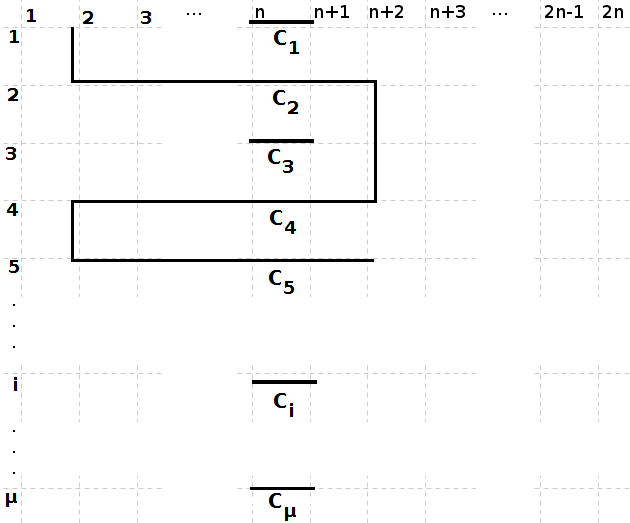
\includegraphics[width=8cm]{./img/grade3.png}
%clausulaGadgetGFCompletaSBPO
\caption{Representação do caminho $P_2$ correspondendo ao vértice $v_2$ contido nas cliques maximais $C_2, C_4$ e $C_5$}
\label{fig:gradeDemonstracao}
\end{figure}
 
 
 
 \begin{corollary}
 Todo grafo $G$ contendo  $\mu$ cliques maximais admite uma representação $B_{2\mu -1}$-EPG-Helly. %in a grid $Q$ of dimension $(\mu \times 2n)$.
 \end{corollary}
 

\section{Relações e Representações EPG Básicas}
%{The Classes $B_1$-EPG and $B_1$-EPG-Helly}

Nessa seção examinaremos as relações hierárquicas entre algumas classes EPG e EPG-Helly. Em complemento, abordaremos representações $B_1$-EPG de alguns grafos que serão utilizados posteriormente. Primeiro, vamos observar como as classes $B_0$-EPG, $B_0$-EPG-Helly, $B_1$-EPG e $B_1$-EPG-Helly se relacionam, em seguida considramos as representações $B_1$-EPG de $C_4$'s.

Apesar das classes  $B_1$-EPG e $ B_1$-EPG-Helly não coincidirem, ver Lemma~\ref{lem:octaedronaohelly}, o mesmo não ocorre para as classes $ B_0$-EPG e $ B_0$-EPG-Helly, como observado no Lemma~\ref{lem:b0epg}.

\begin {lema} \label{lem:b0epg}
Toda representação $ B_0$-EPG satisfaz a propriedade Helly.
\end {lema}
\begin {proof}
Assuma por contradição que exista um grafo $G$ que admite uma representação $ B_0$-EPG que não satisfaz a propriedade Helly. Então, essa representação possui uma coleção minimal de caminhos mutuamente intersectantes $ \mathcal{P} = \{P_{1}, P_{2}, \ldots, P_{k} \} $ tal que $ P_{1} \cap P_{2} \cap \cdots \cap P_{k} = \emptyset, k \geq 3. $
Por minimalidade, sabemos que  $ \bar{P_1} = \mathcal{P} \setminus \{P_1 \}$, $ \bar {P_2} = \mathcal{P} \setminus \{P_2 \} $ e $ \bar {P_3 } = \mathcal{P} \setminus \{P_3) \} $ são mutuamente intersectantes e satisfazem a propriedade Helly.
Assim, existem os seguintes segmentos distintos $ s_{\bar{P_1}}, s_{\bar {P_2}}, s_{\bar {P_3}}$ associados com a intersecção de caminhos em $ \bar {P_1},  \bar {P_2} $ e $ \bar {P_3} $. Uma vez que a representação não possui caminhos com dobras, então sabemos que os caminhos em  $ \mathcal{P}$ estão sobre a mesma linha.
Sem perda de generalidade, vamos assumir que  $ s_{ \bar {P_1}}, s_{ \bar {P_2}}$ e $ s_{ \bar {P_3}}$ ocorrem da esquerda para a direita nessa ordem. Uma vez que $ s_{\bar {P_3}}$ e $ s_{\bar {P_1}}$ intersectam $ P_2 $, e $ P_2 $ é um caminho sem dobra, então $ P_2$ intersecta $ s_{\bar {P_2}}$. Dessa forma temos uma contradição, pois $ s_{\bar {P_2}} $ intersecta todos os caminhos em $ \mathcal{P}$, contradizendo a hipótese de $ P_1 \cap P_2 \cap \cdots \cap P_k = \emptyset $.
\end {proof}
%%%%%%%%%

\begin{corollary}
A classe $B_0$-EPG coincide com a classe $B_0$-EPG-Helly.
\end{corollary}

Grafos $B_0$-EPG coincidem com a classe de grafos de intervalo. O problema de reconhecimento de grafos de intervalo pode ser resolvido em tempo linear~\cite{booth1976}. Apesar de o problema de reconhecimento de grafos $ B_1$-EPG ser $\mathcal{NP}$-completo \cite {heldt2014}, os grafos $ B_1$-EPG-Helly formam uma subclasse propriamente contida em $ B_1$-EPG. Veja a Figura~\ref{fig:diagramaEPG},  além disso, a complexidade de reconhecimento da classe de grafos $ B_1$-EPG-Helly é um problema em aberto. 

O Lema \ref{lem:octaedronaohelly} mostra que as classes  $ B_1$-EPG e $ B_1$-EPG-Helly são distintas, observe o grafo octaedro $ O_3$, ver Figura~\ref{fig:octaedro}(a) que apresenta uma representação  $B_1$-EPG minimal, a menos de isomorfismos, como na Figura~\ref{fig:octaedro}(b). O grafo octaedro  $ O_3 $ pertence a $ B_1$-EPG mas não pertence a $B_1$-EPG-Helly.

\begin{figure}[htb]	
\center%6.3
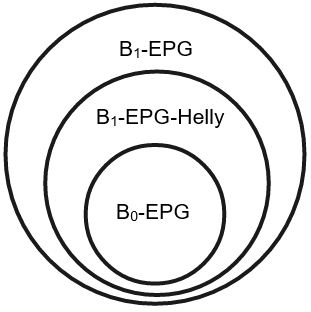
\includegraphics[width=3.5cm]{./img/diagramaClassesEPG.png}
\caption{Diagrama hierárquico de algumas classes  EPG}
\label{fig:diagramaEPG}
\end{figure}



%By the results of \cite{golumbic2009}, in Lemma ~\ref{lem:representacaoC4}, every induced cycle of size 4 in a $ B_1$-EPG  representation  of $C_4$ has only a few possible representations.

\begin{definition} \label{defi:tortasFrame}

Seja $ Q $ uma grade e seja $ (a_1, b),$ $(a_2, b),$ $(a_3, b),$ $(a_4, b)$ uma 4-estrela como retratado na Figura~\ref{fig:piesInGrid}(a). Seja  $ \mathcal{P} = \{P_1, \dots , P_4\}$ uma coleção de caminhos, cada um contendo exatamente duas arestas da $4$-estrela, definimos:

\begin{itemize}
\item Uma \emph{true pie} é uma representação onde cada caminho $P_i$ de $ \mathcal{P} $ forma uma dobra em $b$.

\item Uma \emph {false pie} é uma representação onde dois caminhos distintos $P_i, P_j$  não contém dobra, enquanto os dois caminhos restantes não compartilham aresta. 


\begin{figure}[htb]
  \centering
%segundo bloco de figuras
  \begin{tabular}{c c c c c }
    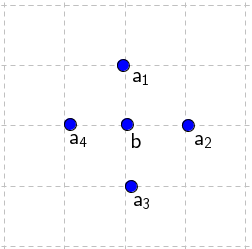
\includegraphics[width=3.5cm]{./img/disposicaoTortaGrid.png}    
    & &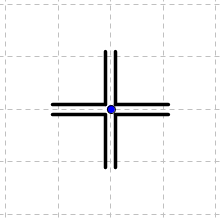
\includegraphics[width=3.5cm]{./img/truePieGrid.png} 
    & &
 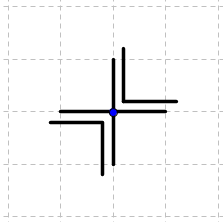
\includegraphics[width=3.5cm]{./img/falsePieGrid.png} \\%[\abovecaptionskip]
    {\footnotesize (a) 4-estrela na grade}  & &  {\footnotesize (b) Torta verdadeira} & & {\footnotesize (c) Torta falsa} %\label{fig:frame}
  \end{tabular}
  \caption{Representações $B_{1}$-EPG do ciclo induzido de tamanho  4 como tortas, com ponto central $b$}\label{fig:piesInGrid}
\end{figure} 

\end{itemize}
\end{definition}
%In both cases the point $b$ is called \emph{center}, see Figures~\ref{fig:piesInGrid}(b) and~\ref{fig:piesInGrid}(c). There are edge-intersections $ (a_1, b), (a_2, b), (a_3, b), (a_4, b)$ called \emph{central rays}, see Figure~\ref{fig:piesInGrid}.

\begin{definition} \label{defi:tortasFrame2}
 Considere um retângulo de qualquer tamanho com os quatro cantos nos vértices  $ (x_1, y_1);$ $(x_2, y_1);$ $(x_2, y_2);$ $(x_1, y_2)$, posicionado como na Figura~\ref{fig:frameInGrid}. Um \emph{frame} é uma representação contendo os 4 caminhos de $\mathcal{P} =  \{ P_1, \dots, P_4\} $, cada um deles tendo uma dobra em uma curva diferente do retângulo, e tal que os subcaminhos $ P_1 \cap P_2, P_2 \cap P_3, P_3 \cap P_4, P_4 \cap P_1 $, compartilham no mínimo uma aresta. Enquanto os subcaminhos  $ P_2 \cap P_4 $ e $ P_1 \cap P_3 $ não compartilham aresta.

\begin{figure}[htb]
  \centering
%segundo bloco de figuras
  \begin{tabular}{c c c c c }
    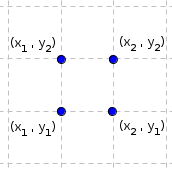
\includegraphics[width=3.5cm]{./img/dispositionFrameInGrid.png}    
    %& &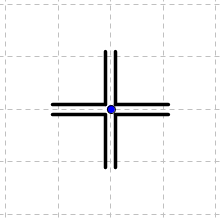
\includegraphics[width=4cm]{./img/truePieGrid.png} 
    & &
 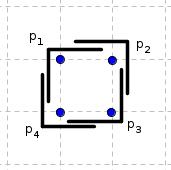
\includegraphics[width=3.5cm]{./img/frameInGrid.png} \\%[\abovecaptionskip]
    {\footnotesize (a) Pontos das coordenadas das dobras de um frame}  
    %& &  {\footnotesize (b) True pie} 
    & & {\footnotesize (c) Caminhos de um frame} %\label{fig:frame}
  \end{tabular}
  \caption{Representações $B_{1}$-EPG de um ciclo induzido de tamanho 4 por frame} \label{fig:frameInGrid}
\end{figure} 
\end{definition}


%% \begin{figure}[htb]	
% \center%6.3
% 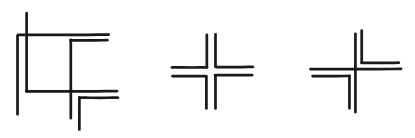
\includegraphics[width=10cm]{./img/representacaociclotam4.png}
% \caption{$B_{1}$-EPG representation of the induced cicle of size 4: frame (in left), true pie (center) and false pie (in right), \cite{golumbic2009}.}

% \end{figure}

\begin{figure}[htb]
  \centering
%segundo bloco de figuras
  \begin{tabular}{c c c c c }
    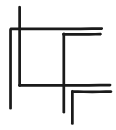
\includegraphics[width=2.3cm]{./img/representacaociclotam41.png}  
    & &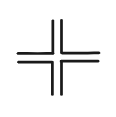
\includegraphics[width=2.5cm]{./img/representacaociclotam42.png} 
    & &
 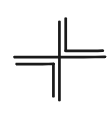
\includegraphics[width=2.5cm]{./img/representacaociclotam43.png} \\%[\abovecaptionskip]
    {\footnotesize (a) Frame}  & &  {\footnotesize (b) True pie} & & {\footnotesize (c) False pie} %\label{fig:frame}
  \end{tabular}
  \caption{$B_{1}$-EPG representation of the induced cycle of size 4}\label{fig:ciclotam4}
\end{figure} 


\begin{lema}\label{lem:representacaoC4}
\cite{golumbic2009} Todo $C_4$ que é um subgrafo induzido de um grafo $ G $ corresponde, em qualquer representação, a uma true pie, a uma false pie, ou a um frame.
\end{lema}
% \begin{prove} Consider a collection of paths $ P = \ {P_1, \dots, P_4}$ of a grid $ Q $ in a $ B_1$-EPG representation of the graph $G$.

% Consider $ C_4 = (v_1, v_2, v_3, v_4) $ that is a chordless 4-cycle in $ G$. Consider $P_i$ the path in $ G $ that corresponds to $v_i $.
% Suppose $ \displaystyle \bigcap _{P_i \in P} P_i \neq \emptyset $, then clearly $ \displaystyle \bigcap _{P_i \in P} P_i = {b} $, for some point $ b $ of the grid. Since each vertex in $ C_4 $ has exactly 2 neighbors, each path $ P_i $ contains exactly two edges of the grid with end point $ b$. Thus, we obtain a star subgraph with center point $ b $ and edges $ (a_1, b), (a_2, b), (a_3, b), (a_4, b)$.
% Without loss of generality, $ P_1 $ contains the edges $ (a_1, b), (a_2, b) $ of the grid. If $ P_2 $ contains $ (a_2, b), (a_3, b) $ or $ (a_1, b), (a_4, b) $, then we get a true pie. Otherwise, $ P_2 $ contains the edges $ (a_2, b), (a_4, b) $ or $ (a_1, b), (a_3, b) $ and we obtain a false pie.

% Otherwise, $ \displaystyle \bigcaP_ {P_i \in P} P_i = \emptyset$. Suppose $ P_1 $ is a path without bend. Each of the $ P_2 $ and $ P_4 $ paths share an edge with $ P_1 $ but do not share a common edge with any other path. If $ P_2 $ and $ P_4 $ do not have a bend, then we get a interval representation of $ C_4 - v_3 $. However, it is not possible to add a $ P_3 $ path with at most of one bend. Similarly, if $ P_2 $ and $ P_4 $ have a single bend, the $ P_3 $ path can not be added either. Therefore, $ P_1 $ has a single bend.

% By symmetry, we assume that all $ P_i $ must has a single bend. Moreover, two paths can not have a bend on a common point in the grid. Thus, we obtain a rectangular subgraph with angles $ (x_1, y_1), (x_2, y_1), (x_2, y_2), (x_1, y_2) $, where $ P_1 $ bends at $ (x_1, y_1) $, $ P_2 $ bends at $ (x_2, y_1) $, $ P_3 $ bends at $ (x_2, y_2) $, and $ P_4 $ bends at $ (x_1, y_2) $, forming a frame.
% $\square$ \end{prove}

\begin{definition}
%A edge is \emph{unnecessary} if its removal keeps the intersections and not intersection of the representation. 
Uma representação $B_k$-EPG é \emph{minimal} quando seu conjunto de arestas não está propriamente contido em outra representação $B_k$-EPG.
%when all unnecessary edges are removed.
\end{definition}

O grafo \textit{octaedro} é o grafo que contém  6 vértices e 12 arestas, retratado na  Figura~\ref{fig:octaedro}(a). A seguir, consideramos  representações do octaedro.

\begin{lema}\label{lem:octaedronaohelly}
O grafo octaedro  $O_3$ possui uma representação $ B_1$-EPG minimal única.
\end{lema}
\begin{proof}
O grafo octaedro $ O_3 $ possui em sua constituição estrutural ciclos induzidos de tamanho  4 ($ C_4$'s). 
Tome um subgrafo $ C_4 $ qualquer do octaedro $ O_3$. O par de vértices não adjacentes do ciclo induzido são gêmeos falsos cuja vizinhança são os vértices pertencentes ao $C_4$ induzido. Cada vértice fora do $C_4$ é adjacente a todos os vértices do $C_4$. Assim quando a representação $ B_1$-EPG do $C_4$ é feita por  frame, nenhum outro caminho da representação de dobra simples pode ser simultaneamente intersectante aos 4 caminhos do frame. Todavia, concluímos que o a estrutura frame não pode ser parte de uma representação de dobra simples do grafo $ O_3$.

Com o mesmo raciocínio, tome uma representação $ B_1$-EPG de $C_4$ agora por true pie ou false pie. Quando adicionamos os caminhos correspondentes a vértices gêmeos falsos, de forma que sejam vizinhos a todos os vértices do $ C_4 $, obtemos $ O_3$, ambas representações convergem para a estrutura apresentada na Figura~\ref{fig:octaedro}(b). 
 \end{proof}

 \begin{figure}[h]
  \centering
  
%segundo bloco de figuras
  \begin{tabular}{@{}c@{} p{1.5cm} @{}c@{} }
   \centering 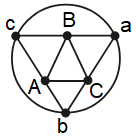
\includegraphics[width=2.5cm]{./img/octaedro.png} & &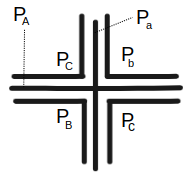
\includegraphics[width=4cm]{./img/representacaoOctaedro.png}  \\[\abovecaptionskip]
    \footnotesize \centering (a) O grafo octaedro $O_3$   & &  \footnotesize(b) Representação $B_1$-EPG do grafo $O_3$
  \end{tabular}

 \caption{O grafo octaedro $O_3$ e sua representação $B_1$-EPG}\label{fig:octaedro}
\end{figure}

Pelo Lema~\ref{lem:octaedronaohelly}, o grafo $ O_3 $ possui uma representação  $B_1$-EPG minimal única, a menos de isomorfismos, como retratado na Figura~\ref{fig:octaedro}(b). Os caminhos $ P_a, P_b $ e $ P_c $  não satisfazem a propriedade Helly, todavia $O_3 \notin B_1$-EPG-Helly. 

\section{Pertinência a $\mathcal{NP}$}

%In this paper we are interested in characterizing the complexity of the $B_1$-EPG-Helly recognition problem, whose formal definition is presented next:
Nessa seção, mostraremos que o problema de reconhecimento de grafos $B_k$-EPG-Helly, onde $k$ é limitado por um polinômio de $|V(G)|$, pertence a  $NP$. O problema pode ser formalmente descrico como segue:

\begin{table}[h!]
\centering
%\caption{My caption}
%\label{my-label}
\begin{tabular}{ll}
\hline \hline
\multicolumn{2}{c}{\sc Reconhecimento $B_k$-EPG-Helly}                         \\ \hline \hline 
\emph{Entrada}: & Um grafo $G$ e um inteiro $k \leq |V(G)|^c$, para alguma constante $c$ fixa.\\
%~ & ~ \\
& \\
\emph{Objetivo:}  & \begin{tabular}[c]{@{}p{11cm}}
Determinar se existe um conjunto de caminhos com $k$-dobras \\ $\mathcal{P} = \{P_1, P_2, \ldots, P_n\} $ em uma grade $ Q $  tal que:\\ 
$\bullet$ \ \ \ $u,v\in V(G)$ são adjacentes em $G$ se e somente se \\ \hspace{0.6cm} $P_u,P_v$ compartilham aresta em $Q$; e\\
$\bullet$ \ \ \ $\mathcal{P}$ satisfaz a propriedade Helly.
\end{tabular} \\ \hline
\end{tabular}
\end{table}


Um certificado (positivo) para o problema {\sc Reconhecimento $B_k$-EPG-Helly} consiste de uma grade $Q$, um conjunto $\mathcal{P}$ caminhos com até $k$-dobras sobre $Q$, que tenham uma correspondência de um-para-um com os vértices do conjunto $V(G)$ de $G$, tal que, para cada par de caminhos distintos $P_i, P_j\in \mathcal{P}, P_i\cap P_j \neq \emptyset $  se e somente se os vértices correspondentes são adjacentes em $G$. Além disso, $\mathcal{P}$ deve satisfazer a propriedade Helly.

Os seguintes conceitos são centrais para nosso propósito.
Uma \emph{aresta relevante} em uma representação $B_k$-EPG é aquela que é aresta de extremidade ou uma aresta de dobra. Portanto, como cada caminho possui no máximo $k$ dobras, então cada caminho pode ter até $2(k+1)$ arestas relevantes, e qualquer representação $B_k$-EPG contém no máximo $2|\mathcal{P}|(k+1)$ arestas relevantes.

A entrada para o algoritmo de verificação do certificado é uma representação $B_k$-EPG, chamemos de $R$, contendo uma coleção de caminhos $\mathcal{P}$, $|\mathcal{P}|=|V(G)|$, onde cada caminho  $P_i \in \mathcal{P}$ é dado pelo seu conjunto de arestas relevantes mais o conjunto de arestas relevantes dos caminhos que intersectam   $P_i$, as arestas relevantes devem ser dadas na ordem que aparecem no caminho. Esse formato de codificação para os caminhos nos permite verificar se cada conjunto de arestas relevantes realmente representa um caminho e se as intersecções correspondem às arestas do grafo em tempo polinomial.

A fim de verificar que a entrada, de fato é um certificado para o problema com tamanho polinomial em $|V(G)|$, temos fazer as seguintes afirmações:

\begin{enumerate}[label=(\roman*)]
\item A sequência de arestas relevantes de um caminho $P_i\in \mathcal{P}$ determina $P_i$ em tempo polinomial; \label{it:bullet1}

\item Dois caminhos  $P_i, P_j \in \mathcal{P}$ são intersectantes se e somente se eles se intersectam em alguma aresta relevante; \label{it:bullet2}

\item O conjunto  $\mathcal{P}$ de arestas relevantes satisfaz a propriedade Helly. \label{it:bullet3}
\end{enumerate}

O Lema a seguir mostra que a condição~\ref{it:bullet1} é válida.

\begin{lema}\label{lem:verify1}
Cada caminho $P_i$ pode ser determinado em tempo polinomial, da considerada sequência de arestas.
\end{lema}

\begin{proof}
É fácil verificar que o item~\ref{it:bullet1} é verdadeiro, considere a sequência de arestas relevantes de algum caminho $P_i\in \mathcal{P}$. Inicie de uma aresta de extremidade de $P_i$. Seja   $t$ a linha (coluna) contendo a última aresta relevante considerada. A próxima aresta relevante  $e'$ na sequência, deve estar contida na linha (coluna) $t$. Se $e'$ é uma aresta de extremidade, o processo está terminado e o caminho tem sido determinado. Ele contém todas arestas entre as arestas relevantes consideradas na sequência.  Caso contrário, se  $e'$ é uma aresta de dobra, a próxima aresta relevante é é a segunda aresta de dobra  $e''$ da mesma dobra, que está contida em alguma coluna (linha) $t'$. O processo continua até que a segunda aresta de extremidade de $P_i$ estar localizada.   

Com o procedimento acima podemos determinar em tempo $O(k+|V(G)|)$, se o caminho $P_i$ contém qualquer dada aresta da grade $Q$. Além disso, a sequência de arestas relevantes de  $P_i$ determina unicamente  $P_i$.
 \end{proof} %$\square$

O lema abaixo mostra que o item~\ref{it:bullet2} é válido.

\begin{lema}\label{lem:relevantEdges}
Seja $R$ uma representação $B_k$-EPG-Helly de $G$, e $P_1, P_2 \in \mathcal{P}$ caminhos de $R$. Então $P_1, P_2$ são caminhos intersectantes se e somente se eles contém uma aresta relevante comum.
\end{lema}


\begin{proof}
Se $P_1, P_2$ contém uma aresta relevante comum não há o que provar. Caso contrário, assuma que $P_1, P_2$ são intersectantes, e mostraremos que eles contém uma aresta relevante comum. Sem perda de generalidade, suponha que $P_1, P_2$ intersectam-se na linha \textit{i} da grade, em uma representação   $B_k$-EPG, digamos $R$. Os seguintes são as possibilidades de casos que podem ocorrer:

\begin{itemize}
\item \textbf{Case 1:} Nem $P_1$ nem $P_2$ contêm dobras na linha \textit{i}. 

Então $P_1$ e $ P_2$  estão inteiramente contidos na linha \textit{i}. Uma vez que eles se intersectam, ou  $P_1, P_2$  se cobrem parcialmente, ou um dos caminhos contém o outro. Em qualquer dessas situações eles intersectam em uma aresta de extremidade comum, que é uma aresta relevante.

\item \textbf{Case 2:} $P_1$ não contém dobras em \textit{i}, mas $ P_2$ contém.

Se alguma aresta de dobra de $P_2$ também pertence a   $P_1$, então $P_1, P_2$  intersectam-se em uma aresta relevante. Caso contrário, uma vez que $P_1, P_2$  intersectam-se, a única possibilidade é que a intersecção contenha uma aresta de extremidade de  $P_1$ ou $ P_2$. Portanto, os caminhos se intersectam em uma aresta relevante.

\item \textbf{Case 3:} Ambos $P_1$,  $P_2$ contém em \textit{i}.

Novamente, se a intersecção ocorre em alguma aresta de dobra de $P_1$  ou $P_2$, o lema segue válido. Caso contrário,  a mesma situação anterior deve ocorrer, ou seja $P_1, P_2$  devem intersectar em alguma aresta de extremidade.
 
\end{itemize}
Em qualquer dos casos, $P_1$ e $P_2$ intersectam-se em alguma aresta relevante.
\end{proof}

Finalmente, provamos o item~\ref{it:bullet3}.

% \begin{enumerate}[label=\roman*]
% \setcounter{enumi}{2}
% \item The set $\mathcal{P}$ of relevant edges satisfies the Helly property. The following lemma shows the above condition.
% \end{enumerate}

\begin{lema}
Seja $\mathcal{P}$ o conjunto de arestas relevantes de uma representação $B_k$-EPG, digamos  $R$, de um grafo  $G$. Podemos verificar que   $R$ é uma representação Helly em tempo polinomial.
\end{lema}
%\setcounter{prove}{2}

\begin{proof}
Seja $\mathcal{T}$ o conjunto de arestas relevantes de $R$. Consideramos cada tripla $T_i$ de arestas de  $\mathcal{T}$. Seja $\mathcal{P}_i$ o conjunto de caminhos de  $R$ contendo no mínimo duas arestas relevantes de $T_i$. Pelo Teorema de Gilmore~\cite{bergeDuchet1975} os caminhos de $\mathcal{P}_i$ contém uma aresta comum se e somente se  $R$  é uma representação Helly.  Pelo Lema~\ref{lem:relevantEdges} eles contêm uma aresta relevante comum. Além disso existe um número polinomial de arestas relevantes, podemos identificar como uma aresta comum em tempo polinomial, e confirmar que $R$ é de fato uma representação Helly. Como o número de triplas também é polinomial, o lema está correto.
 \end{proof} %$\square$

Dos itens (i), (ii) e (iii) podemos concluir o seguinte teorema.

\begin{theorem} \label{teo:npdificuldade}
Uma representação $B_k$-EPG de $G$ pode ser verificada em tempo polinomial, para  $k\leq |V(G)|^c$, para algum inteiro $c$ fixo.
\end{theorem}


\section{$\mathcal{NP}$-Dificuldade}\label{sec:sectionDispositivoClausula}

Agora provaremos que o reconhecimento de grafos   $B_1$-EPG-Helly é $NP$-completo. Para essa demonstração estabelecemos a redução do problema {\sc Positive (1 in 3)-3SAT} definido como segue:

\begin{table}[h!]
\centering
%\caption{My caption}
%\label{my-label}
\begin{tabular}{ll}
\hline \hline
\multicolumn{2}{c}{\sc Positive (1 in 3)-3SAT}                                \\ \hline \hline 
\emph{Entrada}: & \begin{tabular}[c]{@{}p{12.5cm}@{}} Um conjunto $X$ de variáveis positivas; uma coleção $\mathcal{C}=\{C_1,C_2,\ldots,C_m\}$ de cláusulas sobre  $X$ tal que para cada $C_i\in \mathcal{C}$, $|C_i|= 3$.
\end{tabular} \\
 &  \\
\emph{Objetivo}:  & \begin{tabular}[c]{@{}l@{}} %@{}l@{}
Determinar se existe uma atribuição de valores para as variáveis em $ X $\\ de modo que toda cláusula em  $\mathcal{C}$ tem exatamente um literal verdadeiro.
\end{tabular} \\ \hline
\end{tabular}
\end{table}

{\sc Positive (1 in 3)-3SAT } é um problema $\mathcal{NP}$-completo bem conhecido (ver \cite{johnson1979}, problema [L04], pág. 259). {\sc Positive (1 in 3)-3SAT} permanece $\mathcal{NP}$-completo quando o grafo de incidência da fórmula CNF é um grafo planar~\cite{mulzer2008minimum}.

Dado uma fórmula  $F$ que é uma instância de {\sc Positive (1 in 3)-3SAT} apresentaremos uma construção de tempo polinomial de um grafo $ G_F$ tal que  $ G_F $ é $ B_1$-EPG-Helly se e somente se $ F $ é satisfativa. Esse grafo conterá um subgrafo induzido  $ G_c$ com 12 vértices (chamado \emph {clause gadget}) para toda cláusula $ c \in C $, e um subgrafo induzido (\emph {variable gadget}) para cada variável $ x_j$, contendo um vértice especial   $ v_j$, mais um \emph{base gadget}  com 55 vértices adicionais.

%Since a Sun graph $S_4$ whose center is a cycle of size 4 and adding a false twin to each vertex of $S_4$ that is not a member of central induced cycle then we have the graph $H$. 
Utilizaremos um grafo $H$ isomorfo ao grafo ilustrado na Figura~\ref{fig:gadgetBase}, como um  gadget para realizar a prova. Para cada cláusula  $c$ de $F$ do nosso problema alvo, teremos um \emph{clause gadget} isomorfo a $H$, denotado por $G_c$. %The graph $H$ consists of subgraphs whose $B_1$-EPG representations are well known, such as: cycles of sizes 3 and 4.

\begin{figure}[htb]	
\center%6.3
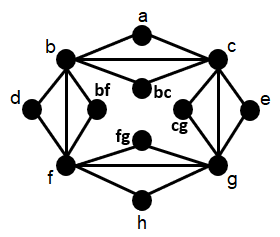
\includegraphics[width=4.5cm]{./img/gadgetBase.png}
\caption{O grafo gadget parcial $H$}
\label{fig:gadgetBase}
\end{figure} 

%\subsection{Definition}\label{sec:reducao}%The problem reduction}

A redução  de uma fórmula $F$ a partir de  {\sc Positive (1 in 3)-3SAT}  para um grafo particular $G_F$ tal que $G_F$ possua uma representação $B_{1}$-EPG-Helly se e somente se $F$ é satisfativa, é dada abaixo.

\begin{definition}\label{sec:reducao}
Seja $F$ uma fórmula na CNF sem literais negativos, em que toda cláusula possua exatamente três literais. O grafo $G_F$ é construído como segue:

\begin{enumerate}
\item Para cada cláusula $C_i \in F$ criar um \textit{clause gadget} $G_{c}$, isomorfo ao grafo $H$;

\item Para cada variável $x_{j}$ criar um \emph{variable vertex} $v_{j}$ que é adjacente aos vértices $a$, $e,$ ou $h$ de $G_c$, quando $x_{j}$ é a primeira, segunda ou terceira variável em $C_i$, respectivamente;

\item Para cada vértice variável $v_{j}$, construir um \emph{variable gadget} formado pela adição de duas cópias de  $H$, digamos $H_1$ e $H_2$, e fazendo $v_j$ adjacente aos vértices dos 2 triângulos $(a, b, c)$ em  $H_1$ e $H_2$.

 %where $v_{j}$ is  adjacent to all vertices of the triangle (a,b,c);%; (c,e,g); (g,f,h); or (b,d,f)) of each $H_1$ and $H_2$; 

%\item The  subgraph induced by \emph{variable vertex}  $v_{j}$, and also $V(H_1)$ and $V(H_2)$ will be called \emph{variable gadget}; 

\item Criar um vértice $V$, que será utilizado como referência vertical para a construção, e adicionar arestas de  $V$ para cada vértice  $d$ nos \emph{clause gadgets};%$d \in V(G_c)$;

\item Criar um grafo bipartido $K_{2,4}$ com um vértice particular $T$ que faz parte do maior conjunto estável desse $K_{2,4}$. Esse vértice é denominado \emph{true vertex}. $T$ é adjacente a todos  $v_{j}$ e também a $V$;

\item Criar dois grafos isomorfos a $H$, digamos $G_{B1}$ e $G_{B2}$. O vértice $T$ é conectado a todos os vértices do triângulo $(a,b,c)$
de cada um;


\item Criar dois grafos isomorfos a $H$, digamos $G_{B3}$ e $G_{B4}$. O vértice $V$ está conectado a todos os vértices do triângulo $(a,b,c)$ de cada um;

\item O subgrafo induzido pelos vértices $V(K_{2,4})$, $T$ e $V$,  $V(G_{B_1})$ e $V(G_{B_2})$, e também por $V(G_{B_3})$ e $V(G_{B_4})$ será denominado como \emph{base gadget}. 
\end{enumerate}
\end{definition}


A Figura~\ref{fig:exemploGrafoGF} retrata como essa construção funciona aplicada sobre uma pequena fórmula. %represents the graph that would be obtained when the previous construction is applied to the formula $ F = (x_1 + x_2 + x_3) \wedge (x_2 + x_3 + x_4) \wedge (x_3 + x_1 + x_4)$.


\begin{figure}[htb]	
\center%6.3
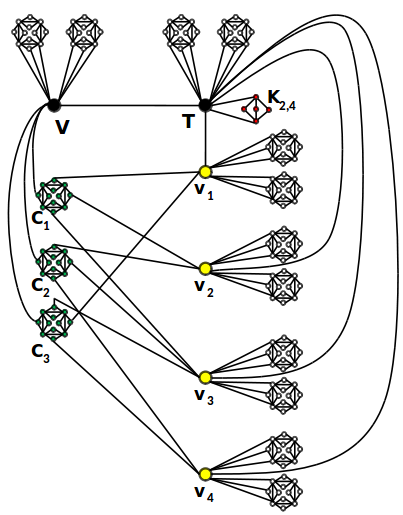
\includegraphics[width=6.5cm]{./img/exemploGrafoGFSBPO4.png}
\caption{O grafo $G_{F}$ correspondendo à fórmula $F=(x_1+ x_2+ x_3) \wedge  (x_2+ x_3+ x_4 )\wedge  (x_3 + x_1 + x_4 )$}
\label{fig:exemploGrafoGF}
\end{figure}


\begin{lema}\label{lem:ida}
Dada uma instância satisfativa $F$ de {\sc Positive (1 in 3)-3SAT}, o grafo  $G_F$ construído a partir de $F$ de acordo com a Definição~\ref{sec:reducao} admite uma representação $B_{1}$-EPG-Helly.
\end{lema}


\begin{proof}

%~\ref{fig:representacaoCaminhos}
Utilizaremos as estruturas  true pie e false pie para representar os  \textit{clause gadgets} $ G_C$, mas a construção poderia ser feita com a estrutura frame sem perda de generalidade, ver Figura~\ref{fig:falseAndTruePie}.  


\begin{figure}[htb]
  \centering
%segundo bloco de figuras
  \begin{tabular}{c c c }
    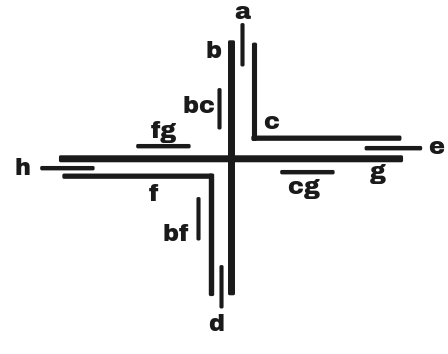
\includegraphics[width=4.5cm]{./img/falsePie.png}  %\label{fig:falsePie} 
    & &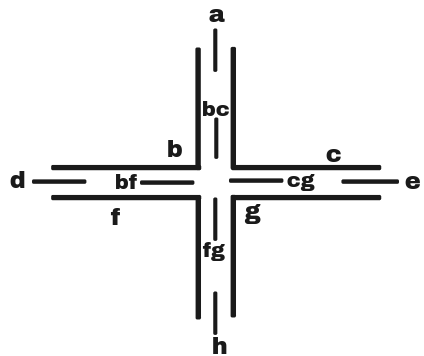
\includegraphics[width=4.5cm]{./img/truePie.png} %\label{fig:truePie}
    \\%[\abovecaptionskip]
    {\footnotesize (a) Baseado em torta falsa}  & &  {\footnotesize(b) Baseado em torta verdadeira}\\
  \end{tabular}
  \caption{Representação de dobra simples  de um dispositivo cláusula isomorfo ao grafo $H$} \label{fig:falseAndTruePie}
\end{figure} 

Os \textit{variable gadgets} serão representados por estruturas como da Figura~\ref{fig:gadgetVariavel}.

\begin{figure}[htb]	
\center%6.3
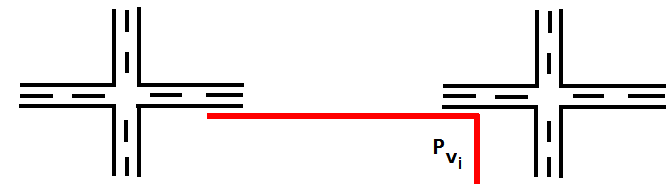
\includegraphics[width=10cm]{./img/gadgetVariavel.png}
%clausulaGadgetGFCompletaSBPO
\caption{Representação de dobra simples de um dispositivo variável}
\label{fig:gadgetVariavel}
\end{figure}


O \textit{base gadget} será representado pela estrutura retratada na  Figura~\ref{fig:gadgetBaseSingleBend}.

\begin{figure}[htb]	
\center%6.3
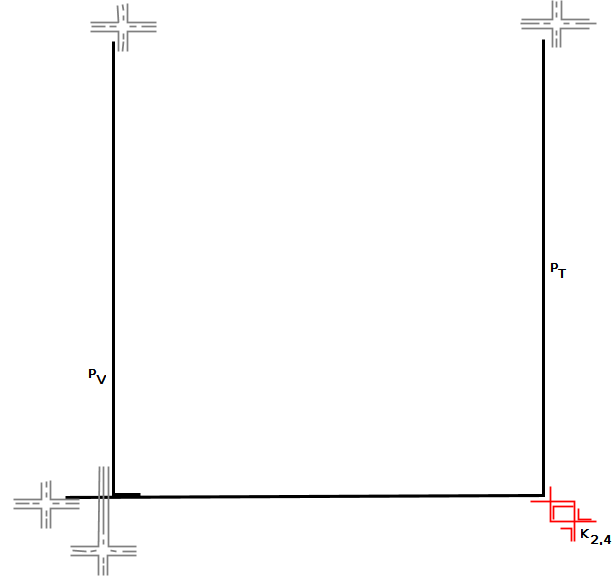
\includegraphics[width=10cm]{./img/gf2.png}
%clausulaGadgetGFCompletaSBPO
\caption{Representação de dobra simples do base gadget}
\label{fig:gadgetBaseSingleBend}
\end{figure}


É fácil ver que as representações dos clause gadgets, variable gadgets, e base gadgets são todas  $B_1$-EPG-Helly. Agora precisamos descrever como essas representações podem ser combinadas de forma a construir uma representação  de dobra simples $R_{G_F}$.

Dada uma atribuição  $A$ que satisfaz  $F$, podemos construir uma representação $R_{G_F}$ que seja  $B_{1}$-EPG-Helly. Primeiro, Fixaremos a estrutura de representação do base gadget na grade para organizar a representação, ver Figura~\ref{fig:gadgetBaseSingleBend}. A seguir inserimos os  variable gadgets com a seguinte regra: se a variável $x_i$ relacionada ao caminho   $P_{v_i}$ tiver atribuição  \textit{True}, então a adjacência entre o caminho $P_{v_i}$ com $P_{T}$ é horizontal, e vertical caso contrário. Por exemplo, uma atribuição  $A=\{x_1=False; x_2=False;x_3=True; x_4=False\}$  para as variáveis da fórmula  $F$ que gerou o gadget $G_F$ da Figura~\ref{fig:exemploGrafoGF}, nos dará um representação de dobra simples (base gadget + variables gadget) de acordo com a  Figura~\ref{fig:gadgetBasePlusVariables}(a). 

Quando a fórmula  $F$ de {\sc Positive (1-in-3)-3sat} possui cláusulas cujo formato de atribuição é $(False, True, False)$ ou $(False, False, True)$ então usaremos false pie para representar essas cláusulas, mas quando a cláusula tem formato  $(True, False, False)$ utilizaremos  true pie para representar essa cláusula. Para inserir um  \textit{ clause gadget} $G_{C}$, introduziremos uma linha horizontal$l_{h}$ na grade entre as linhas horizontais usadas pelos caminhos para as duas false variables em $ C $. Então conectaremos o caminho $P_{d_{c_i}}$ de $G_{C_i}$ em $P_{V}$ verticalmente usando a dobra de  $P_{d_{c_i}}$. No entanto, introduziremos uma linha vertical $ l_{v}$, na grade, entre a linha vertical da grade usada por $P_{V}$ e o caminho para  a true variable em $C_i$, i.e. entre $P_{V}$ e o caminho representando a variável  $x_j \in C_i$. Onde  $l_{h}$  e $l_{v}$ cruzarem, nesse ponto iremos inserir o center do  \textit{clause gadget} como pode ser visto na Figura~\ref{fig:gadgetOnePie}(b). Uma construção completa dessa representação de dobra simples para  $G_F$ pode ser verificada na 
Figura~\ref{fig:gadgetFormulaCompletaPies}.%~\ref{fig:clausulagadgetgf}. 

\begin{landscape}
\begin{figure}[h]
  \centering
%segundo bloco de figuras
  \begin{tabular}{p{10cm} p{2cm} p{10cm}}
   \centering 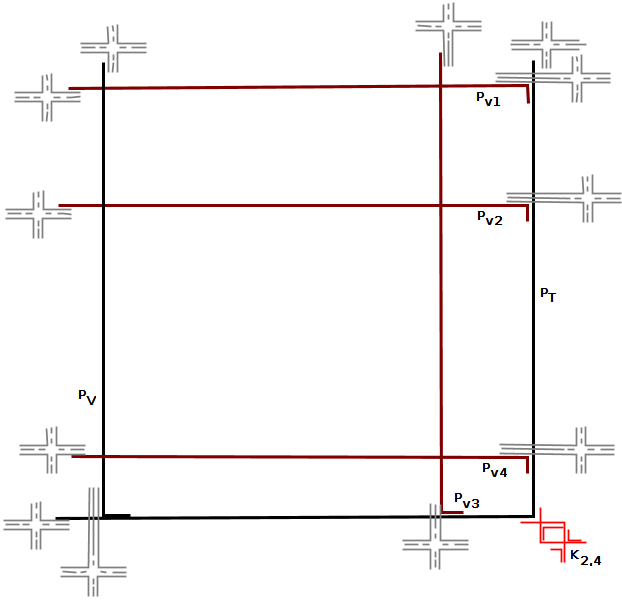
\includegraphics[width=10cm, left]{./img/gf3.png} & & 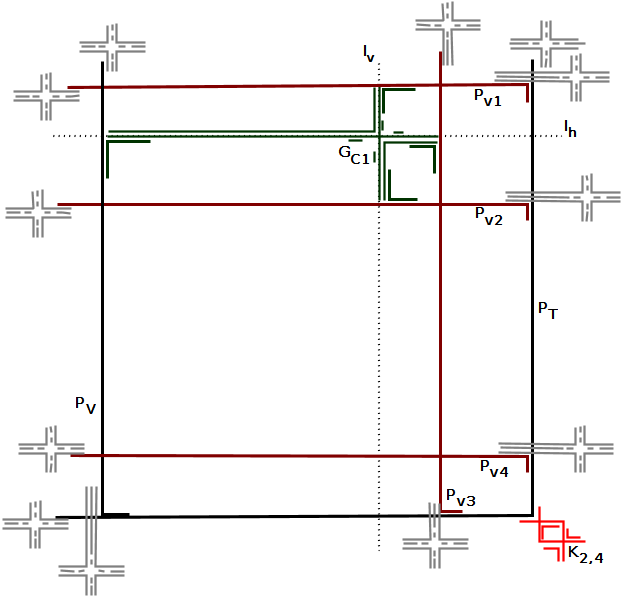
\includegraphics[width=10cm, left]{./img/formulaCompletaGFonePiePlusLines.png} \\  
  [\abovecaptionskip]
    \footnotesize \centering (a) Representação com dispositivos cláusula omitidos & & \footnotesize(b) Representação  com  $G_{C_1}$  associado com a cláusula $(x_1+x_2+x_3)$ em destaque \\
  \end{tabular}

 \caption{Representação de dobra simples dos dispositivos base e variáveis associados com as atribuições $x_1=False, x_2=False, x_3=True, x_4=False$} \label{fig:gadgetOnePie} \label{fig:gadgetBasePlusVariables}
\end{figure}
\end{landscape}


\begin{figure}[htb]	
\center%6.3
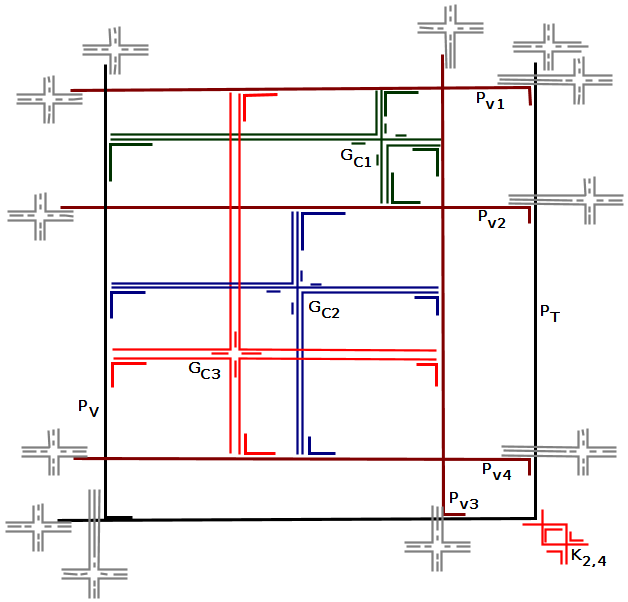
\includegraphics[width=10cm]{./img/formulaFGCompletaPies.png}
%clausulaGadgetGFCompletaSBPO
\caption{Representação de dobra simples de $G_F$}
\label{fig:gadgetFormulaCompletaPies}
\end{figure}


Note que quando juntamos todas essas representações  dos  gadgets que formam $ R_{G_F} $ não há inserção de mais dobras nos caminhos que já possuiam dobra, então a representação necessariamente permanece sendo uma representação  $ B_1$-EPG válida. Nos resta mostrar que ela satisfaz a propriedade Helly. 

Uma forma simples de verificar que $ R_{G_F} $ satisfaz a propriedade Helly é notar que o grafo particular  $G_F$ nunca forma triângulos entre variable, clause, e base gadgets. Assim, qualquer triângulo de  $G_F$ está contido nos variable, clause ou base gadget. Como usamos somente representações  $B_1$-EPG-Helly desses gadgets, $ R_{G_F} $ permanece uma representação $B_1$-EPG-Helly de $G_F$.
 \end{proof}

%\cleardoublepage
%\newpage

A seguir consideramos a conversão. Tome uma representação $R$ de $G_F$ que seja $B_1$-EPG-Helly.

%To complete the proof of $NP$-hardness we will  present some considerations related with the single bend representation of gadgets that form the graph $G_F$. The way all gadgets can be drawn makes it possible to recover the formula that generated $G_F$ and a $True-$assignment for it. The following proofs help us understand the construction of a representation to $G_F$.  

\begin{definition}
Seja $H$ o grafo mostrado na  Figura~\ref{fig:gadgetBase}, tal que um 4-ciclo $H[\{b, c, f, g \}]$ corresponde em $R$ a uma estrutura de false pie ou true pie, então:

\begin{itemize}
\item O \emph{center} é o único ponto da grade dessa representação que está contido em todo caminho representando o 4-ciclo $ \{b, c, f, g \}$; \label{lab:lab1}

\item Um \emph {central ray} é uma aresta-intersecção entre dois dos caminhos correspondendo aos vértices $ b, c, f, g$, respectivamente.
\end{itemize}
\end{definition}


Note que toda representação $B_1$-EPG de um $C_4$ satisfaz a propriedade Helly, ver Lema~\ref{lem:representacaoC4}, e os triângulos possuem $B_1$-EPG representações que satisfazem a propriedade Helly, e.g. a retratada na Figura~\ref{fig:trianguloepgRepresentacao}(b). O grafo $H$ é composto por um 4-ciclo,  $C_4^{H}=H[b, c, f, g]$ e oito triângulos de tamanho 3, que são $(a,b,c);$ $(b,c,bc);$ $(c,e,g);$ $(c,g,cg);$ $(f,g,h);$ $(f,g,fg);$ $(b,d,f);$ $(b,f,bf).$

Como $C_4^{H}$ é um grafo que possui representações bem conhecidas (ver Lema~\ref{lem:representacaoC4}), então podemos iniciar o desenho da representação $B_{1}$-EPG-Helly de $H$ dessas estruturas. As  Figuras~\ref{fig:falsepietruepieframe} retratam possibilidades de representações para $H$.

Se um $C_4^{H}$ é representado por true pie ou false pie, então os caminhos $P_b, P_c, P_f, P_g$ compartilham um ponto central da representação. Por outro lado, se  $C_4^{H}$ é representado por um frame então as dobras dos caminhos correspondem às quatro distintas curvas de um retângulo, i.e. todos os caminhos representando  vértices de um $C_4^{H}$ possuem pontos de dobra distintos, ver~\cite{golumbic2009}.

A seguir examinaremos o uso da estrutura frame.

%Due asymmetric representations, the frame structure needs to be studied in more detail. Next we will show some constraints of this structure. % in which allow us to consider it. %as gadget in the demonstration.

\begin{proposition}\label{lem:direcoesdiferentes}
Em uma representação $B_1$-EPG de um $C_4$ isomorfa a um frame, todo caminho  $P_i$ que representa um vértice do $C_4$ intersecta exatamente dois outros caminhos $P_{i-1}$ e $P_{i+1}$ do frame, de modo que uma das intersecções é vertical e a outra é horizontal. %where one of them is vertical and another is a horizontal intersection.
\end{proposition}

\begin{proof}
A prova é imediata, pela definição de frame.
 \end{proof}

\begin{proposition}\label{lem:mesmaretasuporte}
Dada uma representação $B_1$-EPG-Helly de um grafo $G$ que possui um $C_4$ induzido cuja representação é isomorfa a um frame. Se existe um vértice $v$ de $G$, fora desse $C_4$, que é adjacente a exatamente dois vértices consecutivos desse $C_4$, então o caminho representado por  $v$ possui uma aresta comum com os caminhos representando ambos vértices do $C_4$.% of $v$ into such .  
\end{proposition}

\begin{proof}
Por suposição, $G$ possui um triângulo contendo  $v$ e dois vértices de um $C_4$ representado por frame. Além disso, o caminho representando  $v$ compartilha no mínimo uma aresta que é intersectante aos caminhos que representam seus vizinhos, caso contrário a representação não satisfaz a propriedade Helly.
 \end{proof}

%\cleardoublepage

Pela Proposição~\ref{lem:direcoesdiferentes} e Proposição~\ref{lem:mesmaretasuporte} podemos concluir que para todo vértice   $v_i \in V(H)$ tal que $v_i \neq V(C_4^{H})$, quando usamos um frame para representar o $C_4^{H}$, $P_{v_i}$ terá no mínimo uma aresta-intersecção comum ao par de caminhos representando seus vértices vizinhos em $H$. 
A Figura~\ref{fig:falsepietruepieframe}(c) retrata uma possível representação $B_{1}$-EPG-Helly de $H$. 
Note que ao aplicarmos operações de rotação e espelhamento, mantemos a representação $B_1$-EPG-Helly de $H$.
%On this $B_{1}$-EPG-Helly representation presented we can apply rotation and mirroring operations, because these operations do not change the structure. We can also a change the direction of the bend (see Figure~\ref{fig:falsepietruepieframe}(c) and Figure~\ref{fig:outraRepresentacaoFrame}), but also adjust other paths if needed, so as to not change the intersections between the paths.

\begin{definition}
Em uma representação de dobra simples de um grafo  $C_4$ isomorfo a um frame, os caminhos representando vértices consecutivos no  $C_4$ são chamados \emph{consecutive paths} e o segmento que corresponde à intersecção entre dois caminhos consecutivos é chamado \emph{side intersection}.  
\end{definition}

\begin{lema}\label{lem:2vertical2horizontal}
Em qualquer representação minimal de dobra simples de um grafo isomorfo a $H$ existem dois caminhos em   $\{P_a, P_e, P_d, P_h \}$ que tem direção horizontal e os outros dois caminhos possuem direção vertical.
\end{lema}

\begin{proof}
Se o $C_4^{H} = [b,c,f,g]$ é representado por uma true pie ou false pie então cada caminho do  $C_4^{H}$ compartilha dois central rays com dois outros caminhos do  $C_4^{H}$, onde cada central ray corresponde a um par de vértices consecutivos no $C_4^{H}$.

Como os vértices  $a, e, d, h$ são adjacentes a pares de vértices consecutivos no $C_4^{H}$ então os caminhos $P_a, P_e, P_d, P_h$ tem que se posicionar em cada um dos diferentes central ray,  2 estão na direção horizontal e 2 estão na direção vertical.

Se o $C_4^{H}$ é representado por um frame então cada caminho do $C_4^{H}$ possui uma dobra posicionada em uma curva do frame. No frame, o relacionamento de adjacência de pares de vértices consecutivos no $C_4^{H}$ é representado pela intersecção dos caminhos que constituem o frame. Assim, como um frame possui duas partes da direção vertical e duas partes na direção horizontal, então existem dois caminhos em $\{P_a, P_e, P_d, P_h\}$ que possuem direção vertical e dois caminhos que possuem direção horizontal.
 \end{proof}

\begin{corollary}
 \label{coro:paresMesmoSegmento}
Em qualquer representação minimal de dobra simples de um grafo isomorfo a $H$, os seguintes caminhos estão sobre o mesmo central ray ou side intersection: %$P_a$ and $p(bc)$; $p(e)$ and $p(cg)$; $p(h)$ and $p(fg)$; $p(d)$ and $p(bf)$.

\begin{itemize}
\item $P_a$ e $P_{bc}$;
\item $P_e$ e $P_{cg}$;
\item $P_h$ e $P_{fg}$;
\item $P_d$ e $P_{bf}$.
\end{itemize}
\end{corollary}

\begin{figure}[htb]
  \centering
%segundo bloco de figuras
  \begin{tabular}{c c c c c }
    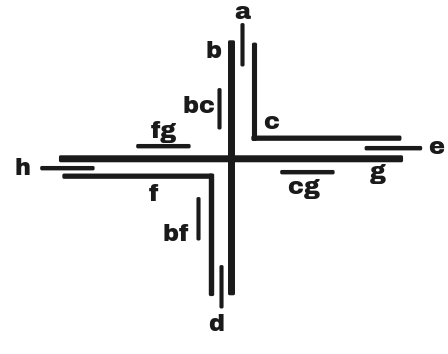
\includegraphics[width=4cm]{./img/falsePie.png}  %\label{fig:falsePie} 
    & &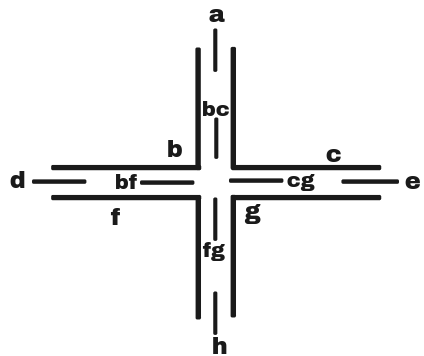
\includegraphics[width=4cm]{./img/truePie.png} %\label{fig:truePie}
    & &
 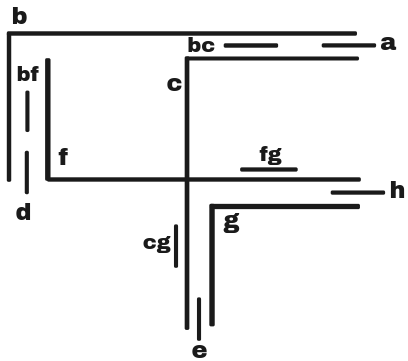
\includegraphics[width=4cm]{./img/frame.png} \\%[\abovecaptionskip]
    {\footnotesize (a) Baseada em false pie}  & &  {\footnotesize(b) Baseada em true pie} & & {\footnotesize (c) Baseada em frame} %\label{fig:frame}
  \end{tabular}
  \caption{Diferentes representações de dobra simples para o grafo  $H$ usando uma  false pie (a), uma true pie (b) e um frame (c) para representar o $C_4^{H}$}\label{fig:falsepietruepieframe}
\end{figure} 

\begin{figure}[htb]	
\center%6.3
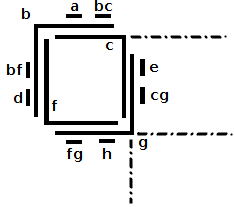
\includegraphics[width=4cm]{./img/outraRepresentacaoFrame3.png}
\caption{Uma representação por frame onde as dobras dos caminhos pontilhados mudaram de sentido}
\label{fig:outraRepresentacaoFrame}
\end{figure}

\begin{definition}
Considere um grafo $G$ e um vértice $v \in V(G)$. Se em uma representação $B_1$-EPG de $G$ as duas arestas de dobra (ou uma aresta de extremidade) do caminho $P_v$ intersecta outros caminhos, então dizemos que  $P_v$ possui uma \emph{dobra obstruída (ou extremidade obstruída)}. 
Em complemento, dada uma $B_1$-EPG representação de $G$ onde $P_v$ possui uma dobra (ou extremidade) obstruída, dizemos que um subconjunto de caminhos \emph{obstruem} uma aresta de dobra (ou uma aresta de extremidade) de  $P_v$ se eles intersectam essa aresta. 
\end{definition}


\begin{fac} \label{fact:k24facts}
Em toda representação de dobra simples de um $K_{2,4}$, o caminho representando cada vértice do maior conjunto estável tem dobra em uma  false pie (ver mais em~\cite{Asinowski2009} e~\cite{daniel2014b}).
\end{fac}


\begin{lema}\label{lem:obstrucao}
Em qualquer representação de dobra simples do grafo  $G'$ retratado na  Figura~\ref{fig:extremidadeDobraObstruida}(a), o caminho $P_x$ possui extremidades e dobra obstruídos.
\end{lema}

\begin{proof}
Considere $G'$ consistindo de um vértice $x$, dois grafos isomorfos a  $H$, digamos $ H_1 $ e $ H_2 $, e um grafo bipartido $K_{2,4}$, tal que: $x$ é vértice do maior conjunto estável de $K_{2,4}$; $x$ é adjacente a um ciclo induzido de tamanho 3 de $H_1$, digamos $C_3^{H_1}$, e a um ciclo induzido de tamanho  3 de $H_2$, digamos $ C_3^{H_2}$, ver Figura~\ref{fig:extremidadeDobraObstruida}(a).

Sabemos que os caminhos pertencentes ao maior conjunto estável de um $K_{2,4}$ sempre dobram em uma  false pie, ver Fato~\ref{fact:k24facts}. Além disso $P_x$ é parte do maior conjunto estável desse  $K_{2,4}$, então $P_x$ possui uma \emph {dobra obstruída}, ver Figura~\ref{fig:extremidadeDobraObstruida}(b). 

O vértice  $x$ é adjacente ao $ C_{3}^{H_1}$ e ao $ C_3^{H_2}$, dessa forma o caminho $ P_x $ intersecta os caminhos representando eles. Mas em representações de dobra simples de um grafo isomorfo a $H$ existem pares de caminhos que sempre estão sobre o mesmo segmento de um central ray ou de uma side intersection, ver o Corolário~\ref{coro:paresMesmoSegmento}, e a representação de  $C_{3}^{H_1}$ ( similarmente para $C_3^{H_2})$ possui um desses caminhos. Todavia, existe uma aresta no cnojunto de caminhos que representam  ${H_1}$ ( similarmente em ${H_2}$) que tem uma intersecção de   3 caminhos representando $ C_{3}^{H_1}$ (e $ C_3^{H_2}$), caso contrário a representação não seria Helly, e existe  uma outra aresta distinta no mesmo  central ray ou side intersection que é intersectada por três outros caminhos diferentes onde pelo menos um deles é diferentes dos caminhos correspondentes a $C_{3}^{H_1}$ ( similarmente $C_3^{H_2}$). Assim, em uma representação de dobra simples de  $G'$, os caminhos que representam  $C_{3}^{H_1}$ (similarmente $C_3^{H_2})$ devem intersectar uma aresta de dobra ou uma aresta de extremidade de $P_x$, porque $P_x$ intersecta somente um dos conjuntos de caminhos que estão sobre o mesmo central ray ou side intersection onde  $C_{3}^{H_1}$ ( similarmente $C_3^{H_2})$ está. Como a dobra de   $P_x$ já está obstruída pelo restante da estrutura de $K_{2,4}$, então ${H_1}$ ( similarmente ${H_2}$) deve estar posicionados nas arestas de extremidade de  $P_x$. Isso implica que  $ P_x $ possui uma condição de \emph{extremidades obstruídas} e \emph{dobra obstruída}, ver Figura~\ref{fig:extremidadeDobraObstruida}(b).
\begin{figure}[h]
  \centering
  \begin{tabular}{p{6cm} p{1cm} p{6cm}}
     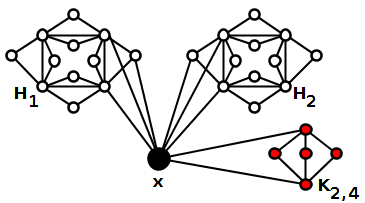
\includegraphics[width=5cm, center]{./img/grafoDobraExtremidadeObstruida2.png} &  &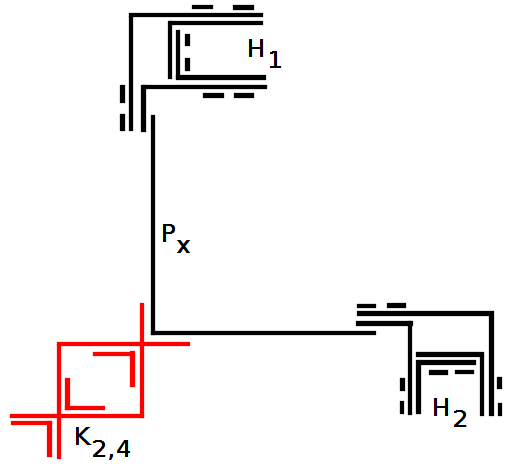
\includegraphics[width=6cm, center]{./img/extremidadeDobraObstruida5.png}  \\%[\abovecaptionskip]
    \footnotesize \centering (a) O grafo $G'$& & \footnotesize \centering (b)Uma representação $B_1$-EPG de $G'$%\\
 %   &&
  \end{tabular}
 \caption{Um exemplo de extremidade e dobra obstruída.} \label{fig:extremidadeDobraObstruida}
\end{figure}
\end{proof}




\begin{definition}
Dizemos que um segmento $s$ está \emph{internally contained} em um caminho $P_x$ se $s$ está contido em $P_x$, e ele não intersecta uma aresta relevante de  $P_x$. 
\end{definition}

% \begin{fac}
% In a single bend representation of a graph, if a path $p(y)$ has an obstructed bend and obstructed extremities, and some path $p(x)$ intersects $p(y)$, but does not intersect paths that obstruct the extremities and the bend edges of $p(y)$, then the intersection between $p(x)$ and $p(y)$ is internally contained into $p(y)$. 
% \end{fac}


\begin{lema}\label{lem:volta}
Se um grafo $G_F$, construído de acordo com a definição  Definição~\ref{sec:reducao}, admite uma representação $B_1$-EPG-Helly, então a CNF-fórmula $F$ associada é uma instância-sim de {\sc Positive (1 in 3)-3sat}.
\end{lema}

% \setcounter{prove}{3}
\begin{proof}
Suponha que $G_F$ possui uma representação $B_1$-EPG-Helly, $R_{G_F}$. A partir de $R_{G_F}$ construiremos uma atribuição que satisfaz $F$. 

Primeiro, note que em toda representação de dobra simples de um $K_{2,4}$, o caminho de cada vértice do maior conjunto estável, em particular $P_{T}$ (em $R_{G_F}$), possui dobras contidas em uma false pie (ver Fato~\ref{fact:k24facts}). 


O vértice  $T$ é adjacente aos vértices de um triângulo de  $G_{B1}$ e $G_{B2}$. Como o $K_{2,4}$ está posicionado na dobra de  $P_{T}$, então em $R_{G_F}$ a representação de $G_{B1}$ e $G_{B2}$ devem ser posicionadas nas extremidades de $P_{T}$, ver Lema~\ref{lem:obstrucao}.   


Sem perda de generalidade, assuma que $P_{V} \cap P_{T}$ é um segmento horizontal em $R_{G_F}$.

Podemos notar em $R_{G_F}$ que: O número de caminhos $P_{d}$ com segmento internamente contido em  $P_{V}$ é exatamente o número de cláusulas em $F$; a intersecção entre cada  $P_{a}, P_{e}, P_{h}$ no  gadget clause e cada caminho $P_{v_j}$ indica as variáveis que compõem a cláusula. Assim, podemos atribuir para cada variável $ x_{j}$ o valor \textit{True} se a aresta intersectante entre $P_{v_j}$ e $P_{T}$ é horizontal, e \textit{False} caso contrário. 


No Lema~\ref{lem:2vertical2horizontal} foi mostrado que qualquer representação minimal $B_1$-EPG de um clause gadget possui dois caminhos em $\{P_{a}, P_{d}, P_{e}, P_{h}\}$ com direção vertical e outros dois caminhos possuem direção horizonal. Além disso $P_{d}$ intersecta $P_{V}$, segue-se que em uma representação de dobra simples de  $G_F$ devemos conectar dois desses caminhos de forma a representar uma atribuição $False$, e exatamente um representará uma atribuição $True$. Assim, mostramos que a partir de $R_{G_F}$ podemos obter uma atribuição para $F$ tal que toda cláusula possui exatamente uma variável com valor $True$.
 \end{proof}

\begin{theorem}
{\sc Reconhecimento de grafos $B_{1}$-EPG-Helly } é NP-completo.
\end{theorem}
\begin{proof}
Pelo Teorema~\ref{teo:npdificuldade} e Lemas~\ref{lem:ida} e~\ref{lem:volta}.
 \end{proof} %$\square$

Dizemos que um grafo $k$-apex é um grafo que pode ser feito planar pela remoção de $k$ vértices. Em complemento, um grafo $d$-degenerate é um grafo em que todo subgrafo possui um vértice de grau no máximo $d$.

\begin{corollary}
 \label{coro:2apexAnd3degenerate}
{\sc Reconhecimento de grafos $B_{1}$-EPG-Helly} é NP-completo sobre grafos $2$-apex e $3$-degenerate.
\end{corollary}

Alguns vértices de  $G_F$ tem representação $B_1$-EPG altamente restritiva. O vértice $T$ possui sua dobra e ambas extremidades obstruídas por seus vizinhos, subgrafos $G_{B1}$, $G_{B2}$ e o restante do grafo $K_{2,4}$. O vértice $V$ e cada  variable vertex $v_i$ deve ter um de seus segmentos internamente contigo em  $T$, e também suas extremidades e dobra obstruídos.  Portanto, o vértice $V$ e cada 
variable vertex possui somente um segmento cada que pode ser utilizado em uma representação EPG para fazer a adjacência deles ao clause gadget. A direção desse segmento, começando pela horizontal ou vertical, pode ser utilizado para representar uma valoração $True$ ou $False$ para as variáveis. Os  clause gadgets, por outro lado, são tais que exatamente duas de suas adjacências aos variable vertices e a $V$ pode ser efetuada com uma intersecção horizontal enquanto as outras duas  devem ser realizadas com intersecção vertical. Se considerarmos a direção utilizada por  $V$ como uma atribuição verdadeira, podemos notar que exatamente uma das variáveis em cada cláusula será $True$ em qualquer possível representação de  $G_F$. Por outro lado, é razoavelmente simples obter uma representação $B_1$-EPG para $G_F$ dada uma atribuição verdadeira para a fórmula $F$.



% \begin{prove}
% It is easy to see that the graphs constructed according to Definition~\ref{sec:reducao} are $3$-degenerate.
% As {\sc Positive (1 in 3)-3SAT} remains NP-complete when the incidence graph of $F$ is planar~\cite{mulzer2008minimum}, from an instance $F$ of {\sc Planar Positive (1 in 3)-3SAT}, by using a planar embedding of the incidence graph of $F$, one can observe that by removing $V$ and $T$ from $G_F$ we obtain a planar graph. Thus, $G_F$ is 2-apex. 
% $\square$ \end{prove}
